\section{Index construction}\label{ch5}
In this chapter we focus on how to construct an inverted index, i.e. the process of \textit{index construction}.

\subsection{Hardware basics}
When building an information retrieval (IR) system, many decisions are based on the characteristics of the computer hardware on which the system runs. The following list provides the hardware basics that are needed to motivate IR systems.

\begin{itemize}
    \item Access to data in \textbf{memory} is much \textbf{faster} than access to data on \textbf{disk}: consequently, we want to keep as much data as possible in memory, especially those data that we need to access frequently. We call the technique of keeping frequently used disk data in main memory \textbf{caching};
    \item When doing a disk read or write, it takes a while for the disk head to move to the part of the disk where the data are located, and \textbf{no data} are being \textbf{transferred} \textbf{during this seek time}. To maximize data transfer rates, chunks of data that will be read together should therefore be stored contiguously on disk;
    \item Operating systems generally \textbf{read} and \textbf{write} entire \textbf{blocks}. Thus, reading a single byte from disk can take as much time as reading the entire block;
    \item \textbf{Data transfers} from disk to memory are handled by the \textbf{system bus}, not by the processor. This means that the processor is available to process data during disk I/O. We can exploit this fact to speed up data transfers by storing compressed data on disk. Assuming an efficient decompression algorithm, the total time of reading and then decompressing compressed data is usually less than reading uncompressed data;
    \item Servers used in IR systems typically have several \textbf{gigabytes} (GB) of \textbf{main memory}, sometimes tens of GB. Available disk space is several orders of magnitude larger;
    \item \textbf{Fault tolerance} is very \textbf{expensive}, so it is much cheaper to use many regular machines rather than one fault-tolerant machine.
\end{itemize}

In particular, Picture \ref{assumptions} shows the hardware assumptions for this chapter.

\begin{figure}[h!]
		\centering
		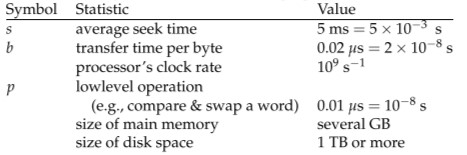
\includegraphics[scale = 1.8]{img/assumptions.jpg}
		\label{assumptions}
        \caption{Hardware assumptions for this chapter}
\end{figure}

\subsection{Blocked sort-based indexing (BSBI)}
The basic steps in constructing an inverted index are represented in Picture \ref{inc_ex}: the first phase is passing through the collection to assemble all the term-docId pairs, then the pairs are sorted and the docIds are organized for each term into a postings list, computing statistics like term and document frequencies. For small collections, all of this can be done in memory, but in this Chapter we analyze some methods for large collections, that require secondary memory storage.

\begin{figure}[h!]
		\centering
		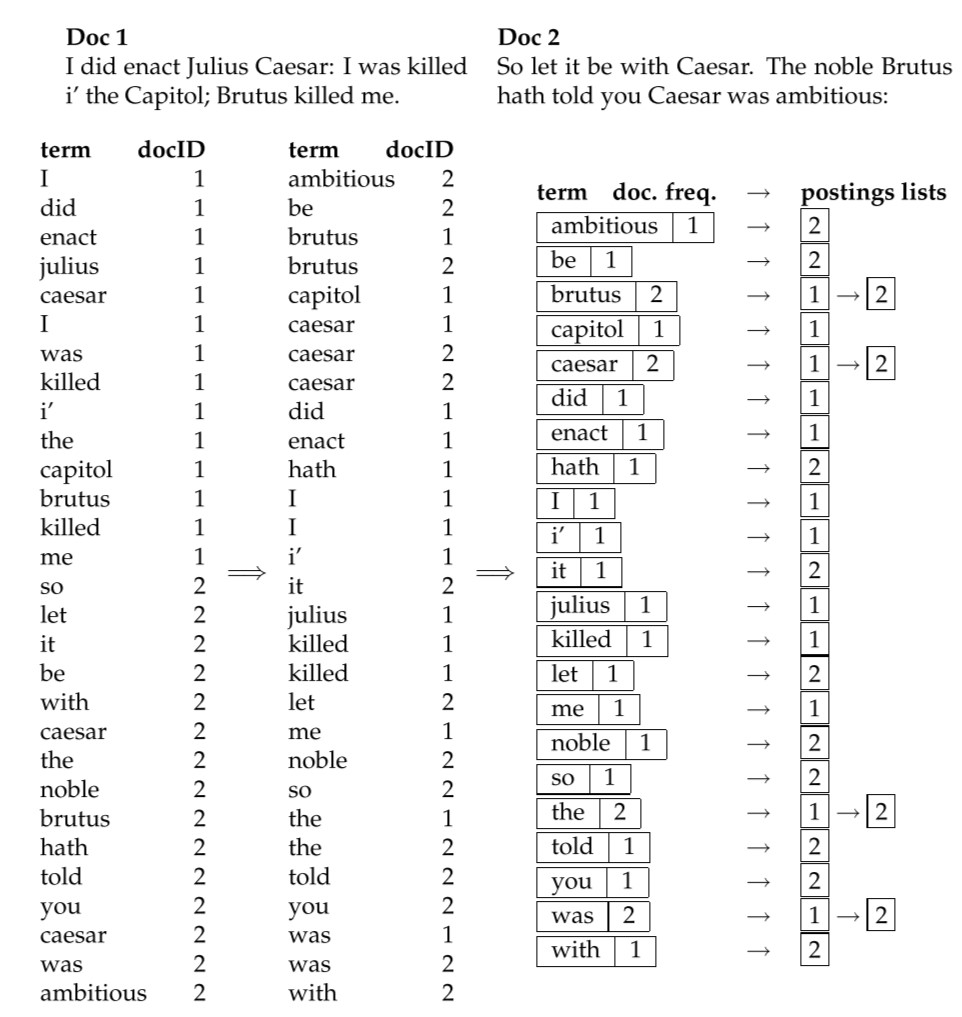
\includegraphics[scale = 0.8]{img/example_inverted index.jpg}
		\label{inc_ex}
\end{figure}

To make index construction more efficient, we represent terms as \textbf{termIDs}, where each termID is a unique serial number, and we work with the \textit{Reuters-RCV1} collection as our model collection in this Chapter, whose statistics are showed in Picture \ref{reuters}.

\begin{figure}[h!]
		\centering
		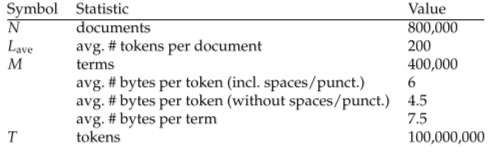
\includegraphics[scale = 1.5]{img/reuters.jpg}
		\label{reuters}
        \caption{Main statistics of \textit{Reuters-RCV1} collection}
\end{figure}

As represented in Picture \ref{inc_ex}, after all the documents have been parsed, the inverted file is sorted by terms. \textit{Reuters-RCV1} contains 100 million tokens, so collecting all termID-docID pairs of the collection using 4 bytes for each pair would require 0.8 GB of storage: clearly, it is not possible to sort them in memory, so we need an \textit{external sorting algorithm}. The main requirement of this algorithm is to minimize the number of random disk seeks during sorting. 

One solution is the \textit{blocked sort-based indexing} algorithm or \textit{BSBI} of Picture \ref{bsbi}. This algorithm:

\begin{enumerate}
    \item Segments the collection into parts of equal size;
    \item Sorts the termID-docID pairs of each part in memory;
    \item Stores the intermediate results on disk;
    \item Merges all intermediate results into the final index.
\end{enumerate}

\begin{figure}[h!]
		\centering
		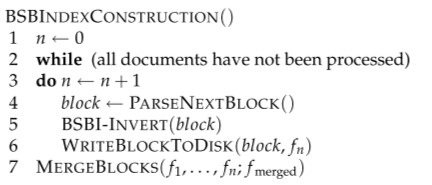
\includegraphics[scale = 1.5]{img/bsbi.jpg}
		\label{bsbi}
        \caption{\textit{BSBI} algorithm}
\end{figure}

Some notes:

\begin{itemize}
    \item The algorithm parses documents into termID–docID pairs and accumulates the pairs in memory until a block of a fixed size is full (function PARSENEXTBLOCK in the code). We choose the block size to fit comfortably into memory to permit a fast in-memory sort;
    \item Then, the termID-docID pairs are sorted;
    \item Next, we collect all termID–docID pairs with the same termID into a postings list, where a posting is simply a docID. The result, an inverted index for the block we have just read, is then written to disk;
    \item Finally, the algorithm simultaneously merges the blocks into one large merged index.
\end{itemize}

If we apply this approach to \textit{Reuters-RCV1} collection, and if we assume that we can fit 10 million termID-docID pairs into memory, we end up with 10 blocks, each of which is an inverted index of one part of the collection. Finally, the blocks are merged into the final index. An example with two blocks is shown in Picture \ref{bsbi example}.

\begin{figure}[h!]
		\centering
		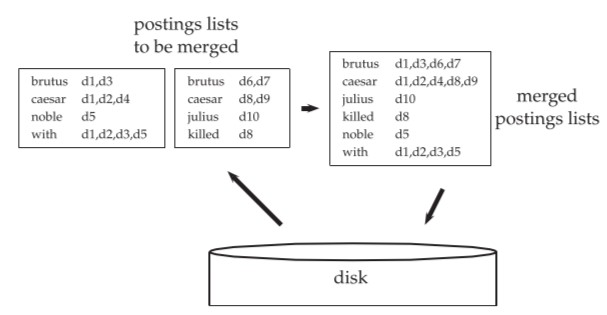
\includegraphics[scale = 1.5]{img/bsbi example.jpg}
		\label{bsbi example}
        \caption{Example of the \textit{BSBI} algorithm}
\end{figure}

One crucial operation of this algorithm is clearly the final \textbf{merge phase}: one possible way to implement it could be by performing a \textbf{binary merge}, but using this strategy we would need to re-write increasingly larger blocks to disk, resulting in a very expensive operation. For this reason, a \textbf{multi-way merge} is preferred, and it consists of opening all the block files simultaneously and maintain small read buffers for the ten blocks we are reading and a write buffer for the final merged index we are writing. By using this technique, we do not perform too many disk seeks, so the algorithm has better performances.

The \textbf{complexity} of \textit{BSBI} algorithm is $\Theta(T log T)$, and it derives by the sorting phase (assuming that we use QuickSort), where $T$ is the number of termID-docID pairs. However, the actual indexing time is dominated by the parsing operation (PARSENEXTBLOCK) and the final merging operation (MERGEBLOCKS). 

Some \textbf{issues} about this algorithm are:

\begin{itemize}
    \item The assumption to use this algorithm is that we're able to keep all the dictionary in memory, and this is not always the case;
    \item Again, the dictionary is needed to produce the mapping from \textit{term} to \textit{termID}: we could also work with term-docID postings, but then the intermediate files would become too large, resulting in a scalable but very slow algorithm.
\end{itemize}

\subsection{Single-pass in-memory indexing (SPIMI)}
The \textit{SPIMI} algorithm is a more scalable alternative to \textit{BSBI} that is based on two key ideas:

\begin{itemize}
    \item It uses terms instead of termID, so no mapping between term and termID is needed across the blocks;
    \item This algorithm does not sort the postings, so the docIDs are generated and assigned sequentially to the documents.
\end{itemize}

Using these two ideas, we can generate a complete inverted index for each block, and then merge them together into one big index. The \textit{SPIMI} algorithm is shown in Picture \ref{spimi}: notice that the part of the algorithm that parses the documents and turns them into term-docID pairs (tokens) is omitted. The algorithm receives in input the token stream, and run until the entire collection has been processed.

\begin{figure}[h!]
		\centering
		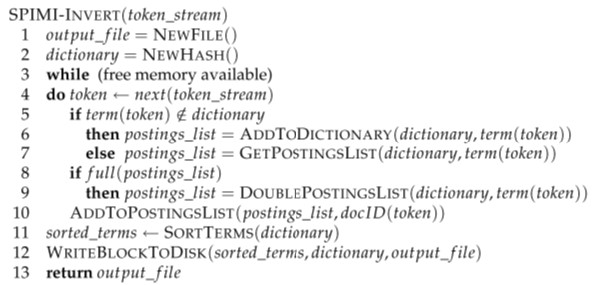
\includegraphics[scale = 1.5]{img/spimi.jpg}
		\label{spimi}
        \caption{\textit{SPIMI} algorithm}
\end{figure}

Some notes:

\begin{itemize}
    \item \textit{Line 4}: each token is processed one at a time;
    \item \textit{Line 5 and 6}: when a term occurs for the first time, it is added to the dictionary and a new empty postings list is created (\textit{Line 6});
    \item \textit{Line 7}: if the term already belongs to the dictionary, the corresponding postings list is retrieved;
    \item \textit{Line 8 and 9}: if the postings list is full, the size is doubled (some memory is wasted);
    \item \textit{Line 10}: the docID of the token is directly inserted into the postings list. Contrary to \textit{BSBI}, where the termID-docID pairs were sorted, here each postings list is dynamic, i.e. its size is adjusted as it grows (\textit{Line 8 and 9}). This approach has two advantages: on the one hand, it is faster since no sorting is required, on the other it saves a lot of memory because the termID of postings need not to be stored;
    \item \textit{Line 11}: when the memory is exhausted, the terms are sorted in order to write the postings lists in lexicographic order, which helps the final merging step;
    \item \textit{Line 12}: the index of the block (dictionary and postings list) is written to disk;
    \item Finally, the blocks are merged (not shown in the picture)
\end{itemize}

Another important feature of this algorithm is \textbf{compression}: both the postings and the dictionary terms can be stored compactly on disk if we employ compression. Compression increases the efficiency of the algorithm further because we can process even larger blocks, and because the individual blocks require less space on disk. We will exploit the compression in the following Chapter. 

The \textbf{time complexity} of \textit{SPIMI} algorithm is $\Theta(T)$, because all operations are at most linear in the size of the collection.

\subsection{Distributed indexing}
Collections are often so large that we cannot perform index construction efficiently on a single machine: Web search engines use \textbf{distributed indexing} algorithms for index construction. The result of the construction process is a distributed index that is partitioned across several machines, either according to term or according to document.

The distributed index construction method we describe in this section is an application of \textbf{MapReduce}, a general architecture for distributed computing, which is designed for large computer clusters (tightly coupled computers that work together closely). Each cluster is composed of cheap commodity machines, or \textit{nodes}, that are able to solve large computing problems, so one the main requirement of \textit{distributed indexing} is to divide the work up into chunks that can be easily assigned and re-assigned to idle nodes in the pool. The \textit{master node} directs the process of assigning jobs to individual nodes, and it is assumed to be "safe", i.e. to be fault tolerant.

The steps of the MapReduce are shown in Picture \ref{map reduce}.

\begin{figure}[h!]
		\centering
		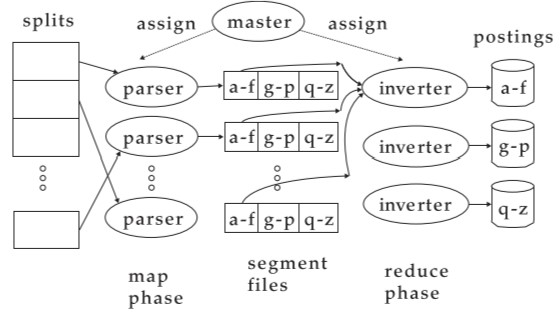
\includegraphics[scale = 1.5]{img/map reduce.jpg}
		\label{map reduce}
        \caption{MapReduce}
\end{figure}

\begin{enumerate}
    \item The input data (a collection of Web pages), is split into \textit{n splits}, where the size of each split is chosen so that the load is is distributed evenly and efficiently among the nodes. Usually, 16 or 64 MB are good choices;
    \item The splits are assigned to the nodes by the \textit{master node} on a ongoing basis: as a machine finishes processing one split, it is assigned to the next one;
    \item The \textit{map phase} consists of mapping splits to term-docID pairs, and since it is the same parsing in \textit{BSBI} and \textit{SPIMI}, we call the machines that execute the map phase \textbf{parsers}. Each parser writes its output to local intermediate files, called \textit{segment files};
    \item In the reduce phase, we would like to have all values for a given key to be stored close together, so that they can be read and processed quickly. This is achieved by \textbf{partitioning the keys} into $j$ term partitions and having the parsers write key-value pairs for each term partition into a separate segment file. In Picture \ref{map reduce}, the term partitions are according to first letter, and $j = 3$. Finally, each parser writes the corresponding segment file, one for each term partition, and each term partition thus corresponds to $r$ segment files, where $r$ is the number of parsers;
    \item The \textit{reduce phase} is performed by the \textbf{inverters}, which collect all values (docIDs) for a given key (termID) into one list. The master assigns each term partition to a different inverter and, as in the case of parsers, reassigns term partitions in case of failing or slow inverters. Each term partition (corresponding to $r$ segment files, one on each parser) is processed by one inverter;
    \item  Finally, the list of values is sorted for each key and written to the final sorted postings list (“postings” in the Picture).
\end{enumerate}

It is important to notice that parsers and inverters are not separate sets of machines, i.e. the same machine can be a parser in the map phase and an inverter in the reduce phase. In general, MapReduce offers a robust and conceptually simple framework for implementing index construction in a distributed environment. By providing a semiautomatic method for splitting index construction into smaller tasks, it can scale to almost arbitrarily large collections.

Picture \ref{map reduce example} shows an example of usage of MapReduce

\begin{figure}[h!]
		\centering
		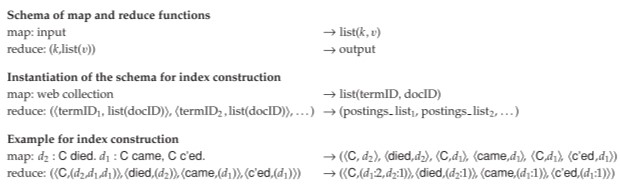
\includegraphics[scale = 1.5]{img/map reduce example.jpg}
		\label{map reduce example}
        \caption{Example of usage of MapReduce}
\end{figure}

\subsection{Dynamic indexing}
Thus far, we have assumed that the document collection is static, but most collections are modified frequently with documents being added, deleted, and updated. This means that new terms need to be added to the dictionary, and postings lists need to be updated for existing terms.

The simplest way to achieve this is to \textbf{periodically reconstruct the index} from scratch. This is a good solution if the number of changes over time is small and a delay in making new documents searchable is acceptable and if enough resources are available to construct a new index while the old one is still available for querying.

If there is a requirement that new documents be included quickly, one solution is to maintain two indexes: a \textit{large main index} and a \textit{small auxiliary index} that stores new documents. The auxiliary index is kept in memory, and the searches are run across both indexes and results merged. Deletions are stored in an invalidation bit vector, and we can then filter out deleted documents before returning the search result. Documents are updated by deleting and reinserting them. The main \textbf{issues} about this strategy may regard the merging phase: however, the merge of the auxiliary index into the main index could be efficient if we keep a separate file for each postings list. In this case, the merge operation would be the same as a simple append, but at the same time we would need to store a lot of files, which is inefficient for the OS. The simplest alternative, which is the one we assume for our purposes, is to store the index as one large file, i.e. a concatenation of postings lists; however, in reality a compromise between the two options is chosen.

Because of this complexity of dynamic indexing, some large search engines adopt a reconstruction-from-scratch strategy. They do not construct indexes dynamically. Instead, a new index is built from scratch periodically.

\subsection{Other types of indexes}

\begin{itemize}
    \item positional indexes;
    \item character n-gram indexes: as the text is parsed, the n-grams are enumerate. Then, for each n-gram we consider the pointers to all dictionary terms that contain it, i.e. the postings.
\end{itemize}
